\documentclass{beamer}
\usetheme{Amsterdam}
\usepackage{adjustbox}
\usepackage{graphicx}
\usepackage{subfig}
\graphicspath{{/Users/evayap/Documents/masters_thesis/presentation/TFL_WIP/plots/}{/Users/evayap/Documents/masters_thesis/ubcdiss_2/chapter3_figure/}{/Users/evayap/Documents/masters_thesis/ubcdiss_2/chapter2_figure/}{/Users/evayap/Documents/masters_thesis/ubcdiss_2/mm_figure/}{/Users/evayap/Documents/masters_thesis/ubcdiss_2/intro_figure/}}
% \usepackage{beamerthemesplit} // Activate for custom appearance
%\setbeamertemplate{caption}[numbered]
%\setbeamerfont{caption}{size=\scriptsize}
\usepackage{caption}
\captionsetup[figure]{labelformat=empty}
\captionsetup[table]{labelformat=empty}
\usepackage{siunitx}
\sisetup{range-phrase = \text{--}}

\title{Germline Variant Calling in Formalin-fixed Paraffin-embedded Tumours}
\author{Eva Yap, MSc. Student}
\date{October 31, 2017}

%%%%%%%%%%%%%%%%%%%%%%%%%%%%%%%%%%%%%%%%%%%%%%%%%%%%%%%%%%%%%%%%%%%%%
\begin{document}

\frame{\titlepage}

%Table of content
\begin{frame}
\frametitle{Overview}
\tableofcontents
\end{frame}

%Begin presentation
%Create overview page
\AtBeginSection[]
{
  \begin{frame}
    \frametitle{Overview}
    \tableofcontents[currentsection]
  \end{frame}
}

%%%%%%%%%%%%%%%%%%%%%%%%%%%%%%%%%%%%%%%%%%%%%%%%%%%%%%%%%%%%%%%%%%%%%
% Background
\section{Background}

\begin{frame}
\frametitle{Germline variants have important clinical implications}
\begin{figure}[t]
    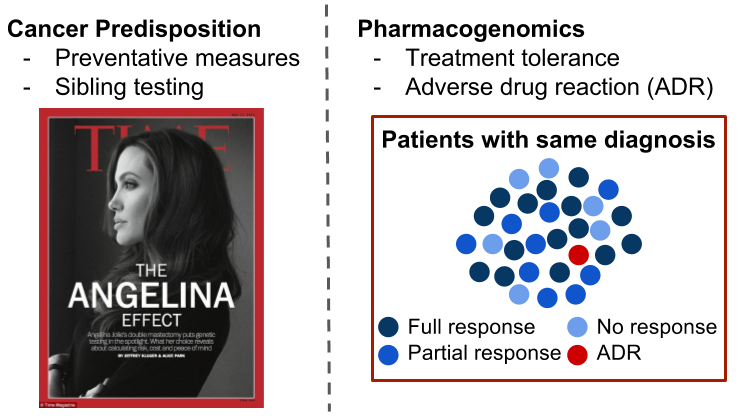
\includegraphics[scale=0.4]{precision_oncology_germline2.png}
\end{figure}
\end{frame}

\begin{frame}
\frametitle{The tumour genome contains germline information}
\begin{figure}[t]
    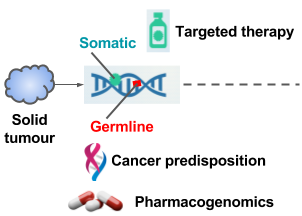
\includegraphics[scale=0.7]{germline_precision.png}
\end{figure}
\end{frame}

\begin{frame}
\frametitle{Clinical tumour sequencing could be a practical, cost-effective approach to provide germline testing}
\centering
\begin{figure}[t]
    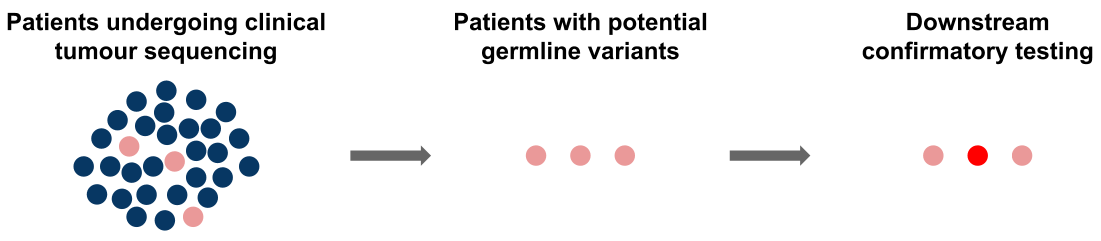
\includegraphics[scale=0.28]{cost_effective_clinical_tumour_sequencing.png}
\end{figure}
\end{frame}

\begin{frame}
\frametitle{Challenge: Distinguishing between germline and somatic variants in the tumour genome}
\begin{figure}[t]
    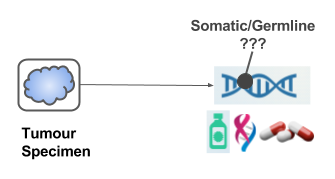
\includegraphics[scale=0.7]{distinguishing_germline_somatic.png}
\end{figure}
\end{frame}

%%%%%%%%%%%%%%%%%%%%%%%%%%%%%%%%%%%%%%%%%%%%%%%%%%%%%%%%%%%%%%%%%%%%%
\section{Research Question}

\begin{frame}
\frametitle{Research question}
Can we accurately identify germline variants in tumour genomes?
\end{frame}

%%%%%%%%%%%%%%%%%%%%%%%%%%%%%%%%%%%%%%%%%%%%%%%%%%%%%%%%%%%%%%%%%%%%%
%%%%%%%%%%%%%%%%%%%%%%%%%%%%%%%%%%%%%%%%%%%%%%%%%%%%%%%%%%%%%%%%%%%%%
% Methods
\section{Methods}

\begin{frame}
\frametitle{Variant allele frequency (VAF)}
\begin{figure}[t]
    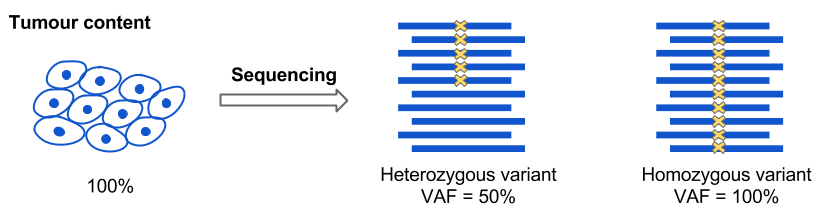
\includegraphics[scale=0.38]{vaf_cells3.png}
\end{figure}
\end{frame}

\begin{frame}
\frametitle{VAF in tumour specimens can deviate from diploid zygosity}
DNA damage induced by formalin (e.g. fragmentation and sequence artifacts)
\begin{figure}[t]
    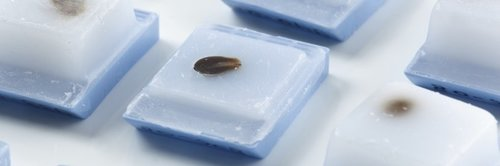
\includegraphics[scale=2]{ffpe_blocks.jpeg}
\end{figure}
\end{frame}

\begin{frame}
\frametitle{Somatic VAF in tumour specimens can deviate from diploid zygosity}
Mixture of tumour and normal cells
\begin{figure}[t]
    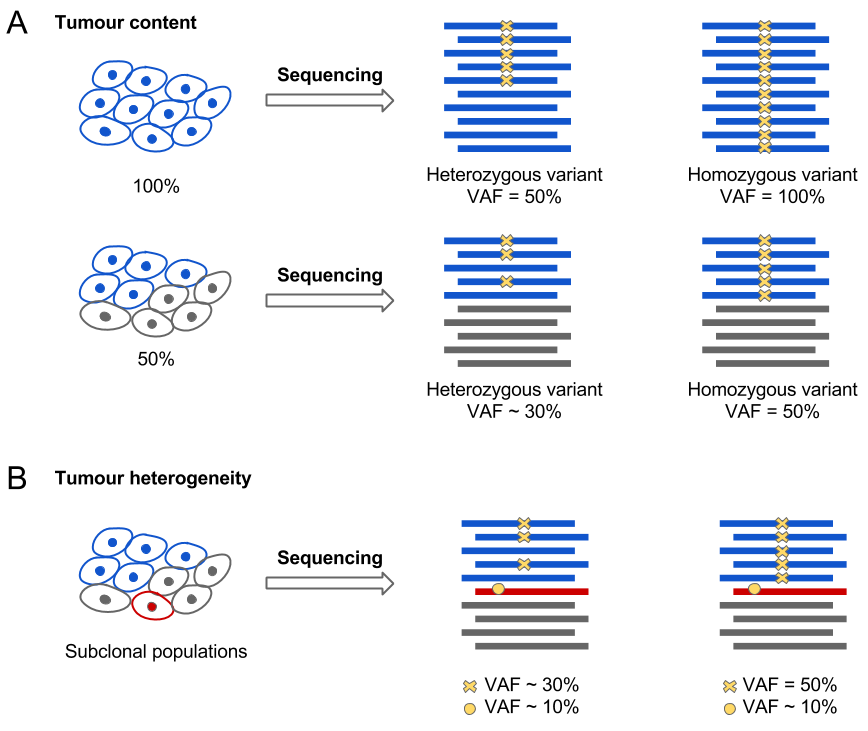
\includegraphics[scale=0.38]{vaf_cells.png}
\end{figure}
\end{frame}

\begin{frame}
\frametitle{Somatic VAF in tumour specimens can deviate from diploid zygosity}
Tumour heterogeneity
\begin{figure}[t]
    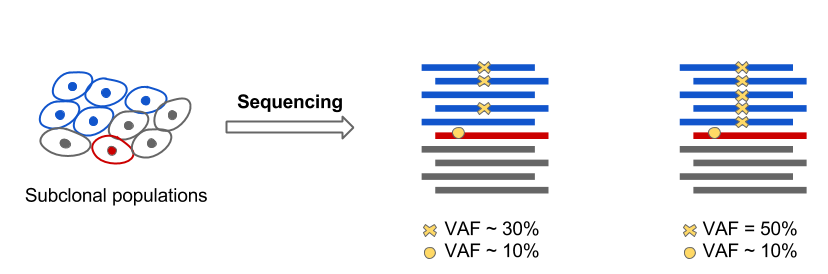
\includegraphics[scale=0.38]{vaf_cells2.png}
\end{figure}
\end{frame}

\begin{frame}
\frametitle{Study Design}
\begin{figure}[t]
    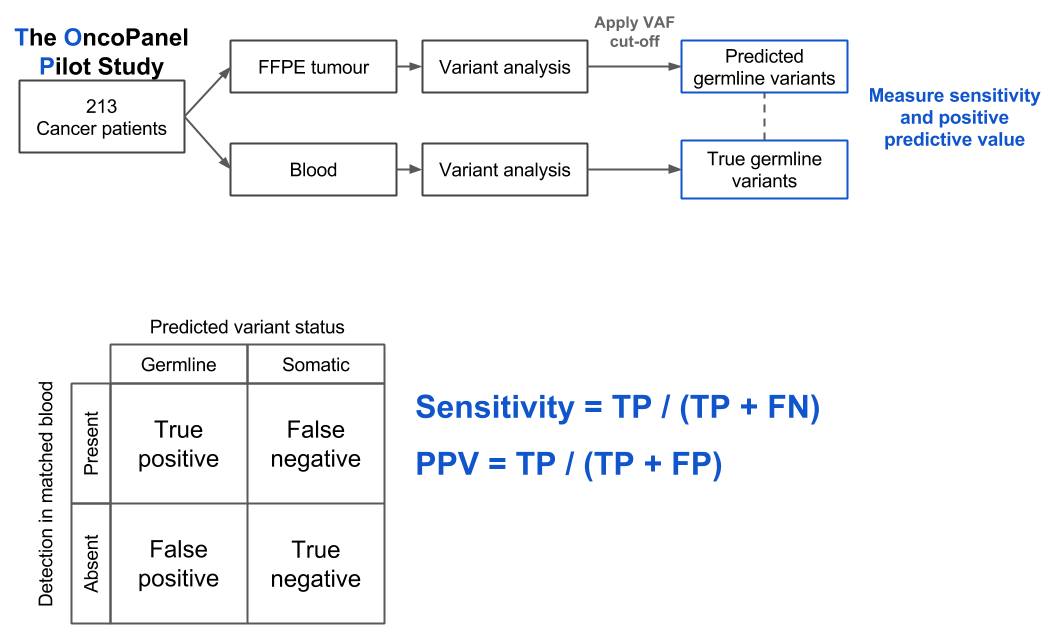
\includegraphics[scale=0.3]{simplify_study_design.png}
\end{figure}
\end{frame}

%%%%%%%%%%%%%%%%%%%%%%%%%%%%%%%%%%%%%%%%%%%%%%%%%%%%%%%%%%%%%%%%%%%%%
%%%%%%%%%%%%%%%%%%%%%%%%%%%%%%%%%%%%%%%%%%%%%%%%%%%%%%%%%%%%%%%%%%%%%
\section{Results}

\begin{frame}
\frametitle{VAF of germline variants in blood and FFPE tumours}
\begin{figure}[t]
    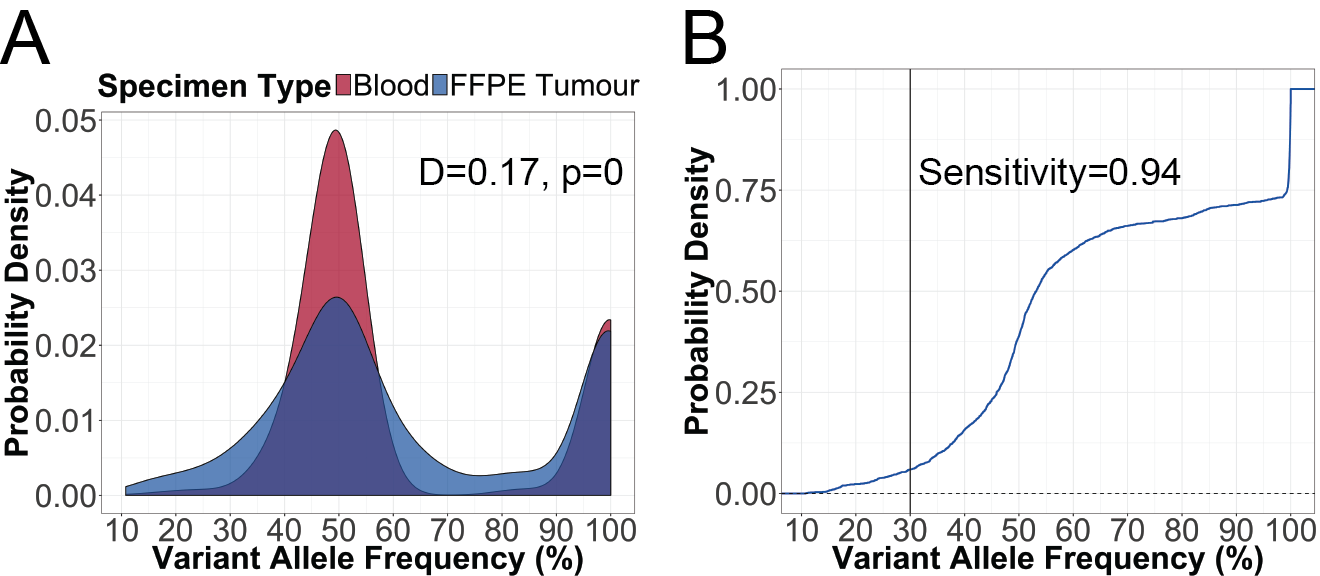
\includegraphics[scale=0.5]{germline_sens_minor.png}
\end{figure}
\end{frame}

\begin{frame}
\frametitle{Sensitivity in detection of germline variants at different VAF thresholds}
\begin{table}
\footnotesize
\centering
      \begin{tabular}{ccc|ll}
        \hline
        VAF (\%) & False Negative & True Positive & Sensitivity & 95\% CI
        \\
        \hline
        10 & 0 & 1981 & 1.0 & 1.0--1.0
        \\
        15 & 13 & 1968 & 0.99 & 0.99-1.0
        \\
        20 & 46 & 1935 & 0.98 & 0.97--0.98
        \\
        25 & 77 & 1904 & 0.96 & 0.95--0.97
        \\
        30 & 117 & 1864 & 0.94 & 0.93--0.95
        \\
        35 & 192 & 1789 & 0.90 & 0.89--0.92
        \\
        40 & 313 & 1668 & 0.84 & 0.83--0.86
        \\
        45 & 458 & 1523 & 0.77 & 0.75--0.79
        \\
				\hline
      \end{tabular} \\
\end{table}
\end{frame}

\begin{frame}
\frametitle{VAF of germline and somatic variants in FFPE tumour}
\begin{figure}[t]
    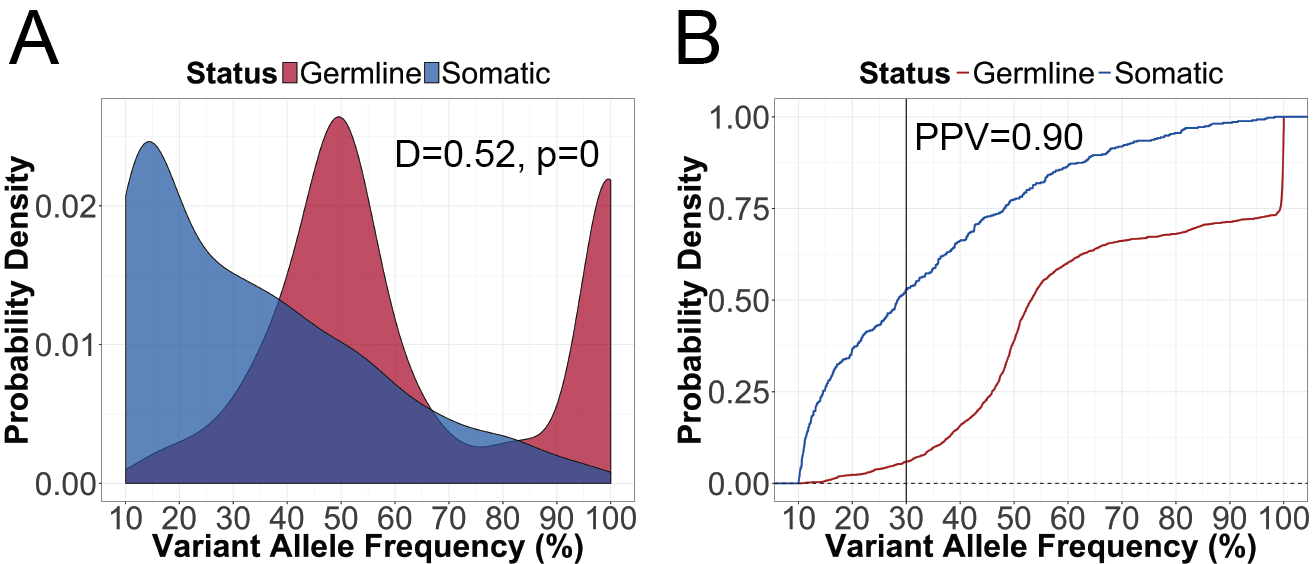
\includegraphics[scale=0.5]{germline_ppv_minor.png}
\end{figure}
\end{frame}

\begin{frame}
\frametitle{High positive predictive value can be achieved for referral of germline variants to downstream confirmatory testing}
\centering
\scriptsize
\begin{table}[H]
\centering
      \begin{tabular}{cccccll}
        \hline
        VAF (\%) & False Positive & True Positive & Total Calls & PPV & 95\% CI
        \\
        \hline
        10 & 431 & 1981 & 2412 & 0.82 & 0.81--0.84
        \\
        15 & 319 & 1968 & 2287 & 0.86 & 0.85--0.87
        \\
        20 & 273 & 1935 & 2208 & 0.88 & 0.86--0.89
        \\
        25 & 245 & 1904 & 2149 & 0.89 & 0.87--0.90
        \\
        30 & 203 & 1864 & 2067 & 0.90 & 0.89--0.91
        \\
        35 & 178 & 1789 & 1967 & 0.91 & 0.90--0.92
        \\
        40 & 146 & 1668 & 1814 & 0.92 & 0.91--0.93
        \\
        45 & 118 & 1523 & 1641 & 0.93 & 0.91--0.94
        \\
				\hline
      \end{tabular} \\
\end{table}
\end{frame}

%%%%%%%%%%%%%%%%%%%%%%%%%%%%%%%%%%%%%%%%%%%%%%%%%%%%%%%%%%%%%%%%%%%%%
% Conclusion
\section{Conclusions}
\begin{frame}
\frametitle{Conclusions}
\begin{enumerate}
\uncover<1->{\item A VAF approach demonstrates high sensitivity and precision at separating between germline and somatic variants.}
\uncover<2->{\item At 30\% VAF threshold, sensitivity for detection of germline variants in FFPE tumour is \textcolor{red}{0.94} and the positive predictive value for referral to downstream confirmatory testing is \textcolor{red}{0.90}.}
\uncover<3->{\item Germline variants could be accurately identified in FFPE tumour sequencing.}
\end{enumerate}
\end{frame}

%%%%%%%%%%%%%%%%%%%%%%%%%%%%%%%%%%%%%%%%%%%%%%%%%%%%%%%%%%%%%%%%%%%%%

\begin{frame}
\frametitle{Acknowledgements}
\begin{columns}[T] % align columns
\begin{column}{.48\textwidth}
Dr. Aly Karsan \\
Dr. Jennifer Grants \\
Dr. Jeremy Parker \\
Dr. Kieran O'Neill \\
Dr. Marion van den Bosch \\
Dr. Rawa Ibrahim \\
Dr. Sergio Martinez-Hoyer \\
Angela Mo \\
Patrick Coulombe \\
Rod Docking \\
Jenny Li \\
Deborah Deng \\
Helen Lin
\end{column}%
\hfill%
\begin{column}{.48\textwidth}
Committee members: \\
Dr. Martin Hirst \\
Dr. Ryan Morin
\\~\\
Centre for Clinical Genomics
\\~\\
Canada's Michael Smith Genome Sciences Centre
\\~\\
Patients from The OncoPanel Pilot study (H14-01212)
\end{column}%
\end{columns}
\end{frame}

\end{document}

\endinput
\begin{frame}
\frametitle{Constraints in the clinic}
\begin{enumerate}
\uncover<1->{\item Financial}
\uncover<2->{\item Time}
\uncover<3->{\item Sample availability}
\end{enumerate}
\end{frame}

\begin{frame}
\frametitle{Challenge 2: Tumour specimens are often formalin-fixed paraffin-embedded}
\begin{figure}[t]
    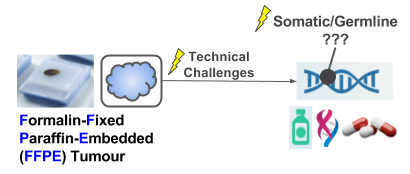
\includegraphics[scale=0.7]{ffpe_technical_challenge.png}
\end{figure}
\begin{enumerate}
\uncover<1->{\item DNA fragmentation}
\uncover<2->{\item Sequence artifacts (e.g. C$>$T/G$>$A transitions)}
\end{enumerate}
\end{frame}

\begin{frame}
\frametitle{Tumour types in the TOP cohort}
\small
\begin{table}
\caption{}
\centering
      \begin{tabular}{lccc}
        \hline
        Cancer Type & Number of Cases & Percentage (\%) \\ \hline
        Colorectal & 97 & 46 \\
        Lung & 59 & 28 \\
        Melanoma & 18 & 8 \\
				Other & 17 & 8 \\
				GIST & 7 & 3 \\
				Sarcoma & 4 & 2 \\
				Neuroendocrine & 4 & 2 \\
				Cervical & 2 & 0.9 \\
				Ovarian & 2 & 0.9 \\
				Breast & 2 & 0.9 \\
				Unknown & 1 & 0.5 \\
        \hline
      \end{tabular}
\end{table}
\end{frame}

\begin{frame}
\frametitle{Cancer-related genes in the OncoPanel}
\scriptsize
\begin{table}
    \caption{}
    \centering
    \begin{tabular}{lll}
    \hline
    Gene & Protein \\
    \hline
    AKT1 & Protein kinase B \\
    ALK & Anaplastic lymphoma receptor tyrosine kinase \\
    BRAF & Serine/threonine-protein kinase B-Raf \\
    EGFR & Epidermal growth factor receptor \\
    HRAS & GTPase HRas \\
    MAPK1 & Mitogen-activated protein kinase 1 \\
    MAP2K1 & Mitogen-activated protein kinase kinase 1 \\
    MTOR & Serine/threonine-protein kinase mTOR \\
    NRAS & Neuroblastoma RAS viral oncogene homolog \\
    PDGFRA & Platelet-derived growth factor receptor alpha \\
    PIK3CA & Phosphatidylinositol-4,5-bisphosphate 3-kinase catalytic subunit alpha \\
    PTEN & Phosphatase and tensin homolog \\
    STAT1 & Signal transducer and activator of transcription 1 \\
    STAT3 & Signal transducer and activator of transcription 3 \\
    TP53 & Tumor protein P53 \\
    \hline
    \end{tabular}
\end{table}
\end{frame}

\begin{frame}
\frametitle{Pharmacogenomic-related genes in the OncoPanel}
\scriptsize
\begin{table}
    \caption{}
    \centering
    \begin{tabular}{llll}
    \hline
    Gene & Protein & Chemotherapy \\
    \hline
    DPYD & Dihydropyrimidine dehydrogenase & 5-FU \\
    GSTP1 & Glutathione S-rransferase pi 1 & Oxaliplatin \\
    MTHFR & Methylenetetrahydrofolate reductase & 5-FU \\
    TYMP & Thymidine phosphorylase & 5-FU \\
    TYMS & Thymidylate synthetase & 5-FU \\
    UGT1A1 & Uridine diphosphate (UDP)-glucuronosyl transferase 1A1 & Irinotecan \\
    \hline
    \end{tabular}
\end{table}
\end{frame}

\begin{frame}
\frametitle{The era of precision oncology}
\begin{figure}[t]
    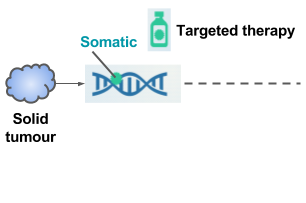
\includegraphics[scale=0.7]{somatic_precision.png}
\end{figure}
\end{frame}

\begin{frame}
\frametitle{BC Cancer Agency's OncoPanel}
\begin{figure}[t]
    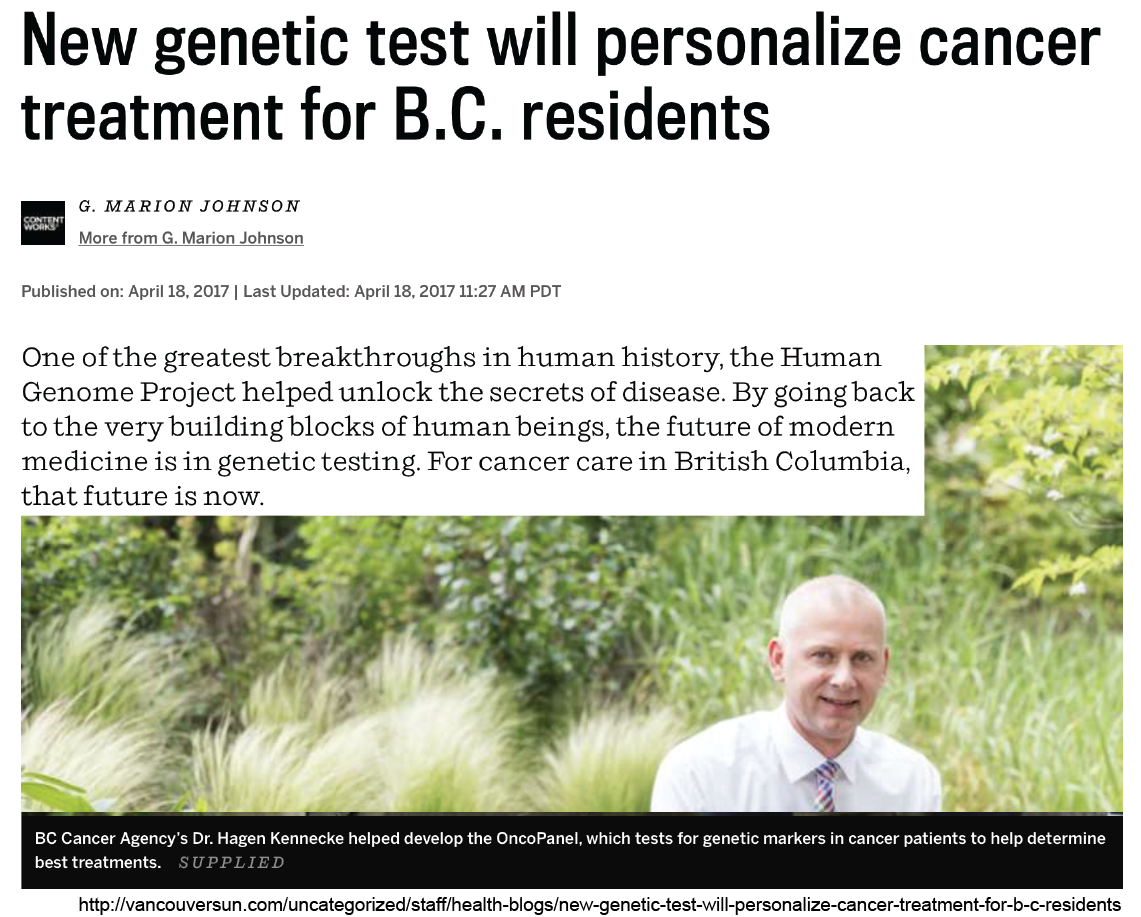
\includegraphics[scale=0.4]{oncopanel_news.png}
\end{figure}
\end{frame}

\begin{frame}
\frametitle{BC Cancer Agency's OncoPanel}
\begin{figure}[t]
    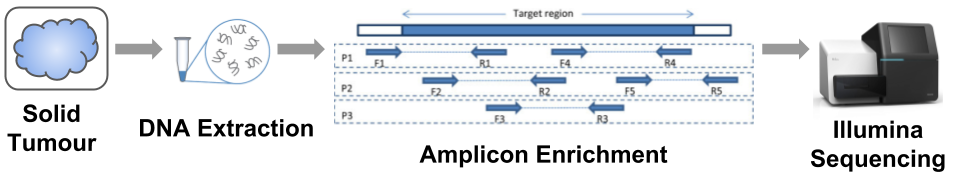
\includegraphics[scale=0.33]{oncopanel_amplicon_sequencing.png}
\end{figure}
\begin{enumerate}
\uncover<1->{\item Targeted massively parallel sequencing panel for solid tumours}
\uncover<2->{\item First gene panel to be available province wide and as part of standard of care}
\end{enumerate}
\end{frame}

\begin{frame}
\frametitle{Acknowledgements}
\begin{figure}[t]
    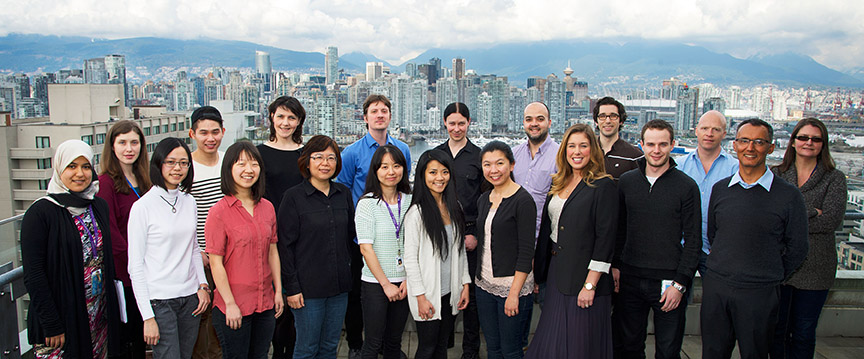
\includegraphics[scale=0.3]{Karsan-Lab_4470_web}
\end{figure}
\end{frame}
